\documentclass{article}

% set font encoding for PDFLaTeX or XeLaTeX
\usepackage{graphicx}
\usepackage{ifxetex}
\usepackage{hyperref}

\ifxetex
  \usepackage{fontspec}
\else
  \usepackage[T1]{fontenc}
  \usepackage[utf8]{inputenc}
  \usepackage{lmodern}
\fi
\title{Actividad 4}
\author{Fisica Computacional 1\\
Corral Valdez Jesus Giovanni\\
Departamento de Física\\
Universidad de Sonora}
\date{}
% Enable SageTeX to run SageMath code right inside this LaTeX file.
% documentation: http://mirrors.ctan.org/macros/latex/contrib/sagetex/sagetexpackage.pdf
% \usepackage{sagetex}


\begin{document}
\maketitle
\clearpage
\section{Introducción}
Como actividad final del curso se nos encargó analizar las mareas de cualquier lugar que quisiéramos. Los datos los obtuvimos de un Centro de Investigación en Ensenada (CICESE, \url{http://redmar.cicese.mx/meteoro/graph/prediccion.php})
\begin{figure}[h]
  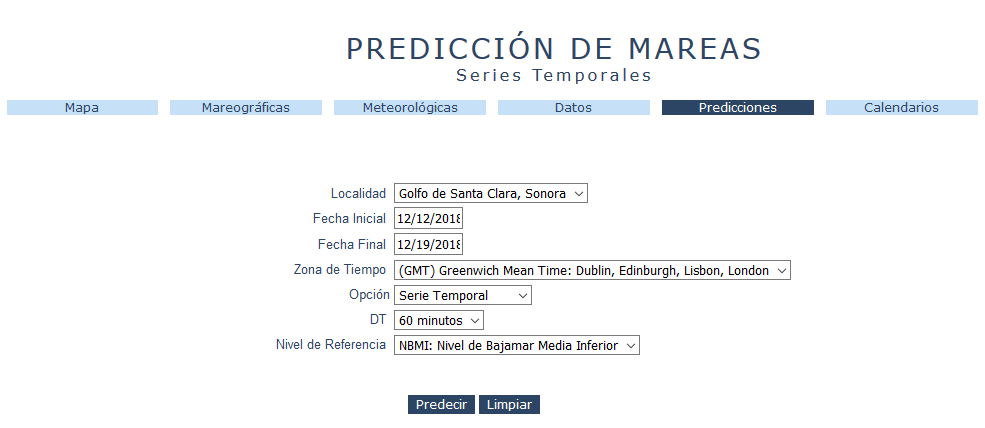
\includegraphics[width=\linewidth]{4-01.png}
\end{figure}


Después de haber importado los datos, se graficarán usando la "Fast Fourier Transform" para poder obtener los constituyentes de nuestras mareas.\\
\begin{figure}[h]
  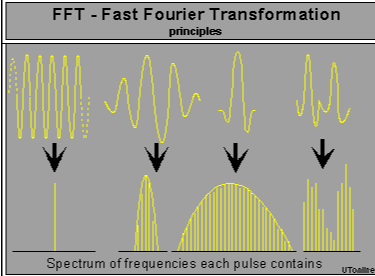
\includegraphics[width=\linewidth]{4-02.png}
\end{figure}

\clearpage
\section{Desarrollo}
1.Se importan las herramientas que estaremos utilizando (notese que ahora se importan cosas relacionadas con la transformada de Fourier que se hará).\\
\begin{figure}[h]
  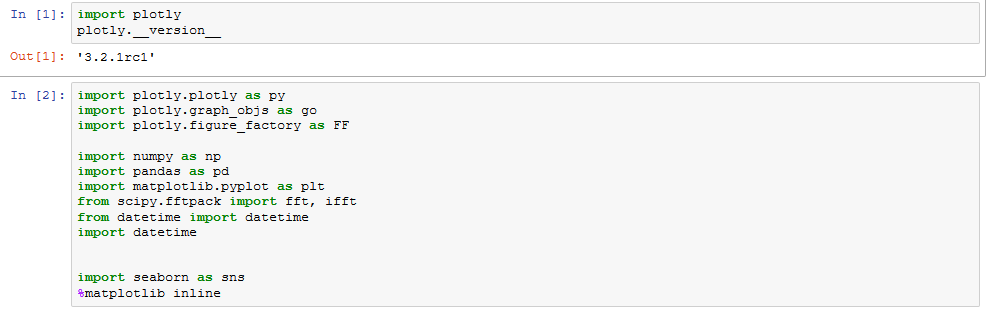
\includegraphics[width=\linewidth]{4-03.png}
\end{figure}

2.Se descargaron los datos de mareas del Golfo de Santa Clara durante el 2018. Despues de adaptarlos a la extensión ".csv" en Excel se leyeron por medio de Pandas.\\
\begin{figure}[h]
  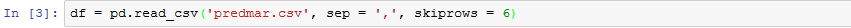
\includegraphics[width=\linewidth]{4-04.png}
\end{figure}
\clearpage
3. Se empezó asignandole nombre a las columnas y se juntó la columna de fecha con la de hora, para crear un solo "datetime" para facilitar la graficación. Se tuvieron que reemplazar algunos caracteres para que esto fuera posible.\\
\begin{figure}[h]
  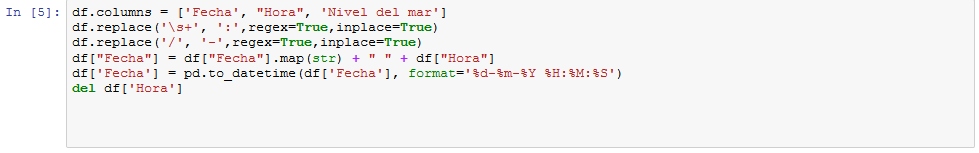
\includegraphics[width=\linewidth]{4-05.png}
\end{figure}

4.Es mas fácil analizar datos de cantidades no tan grandes, por lo que los datos se separaron en intervalos de tres meses y se graficaron por medio de Plotly.\\
\begin{figure}[h]
  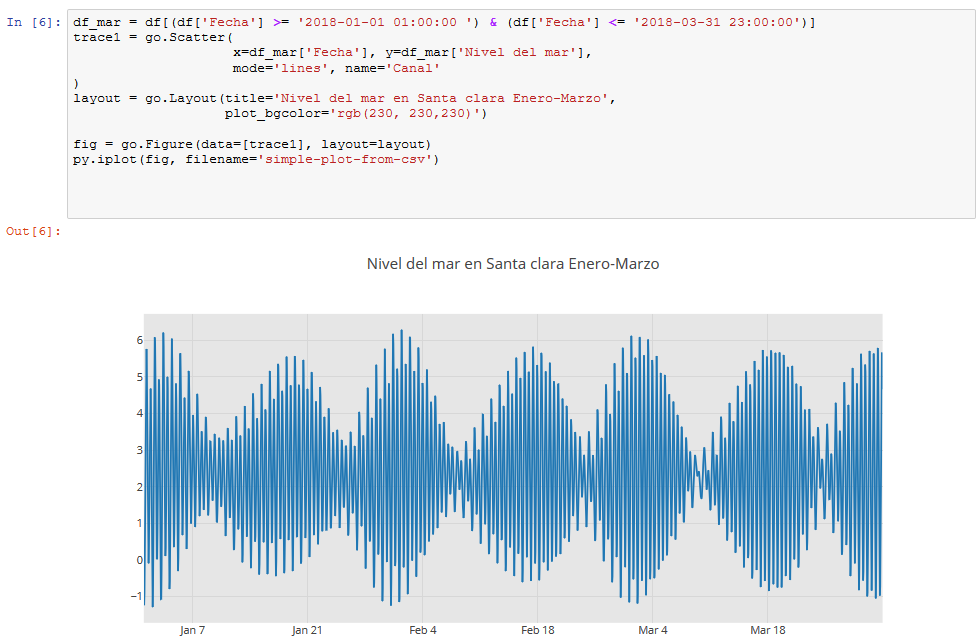
\includegraphics[width=\linewidth]{4-06.png}
\end{figure}
\clearpage
\begin{figure}[h]
  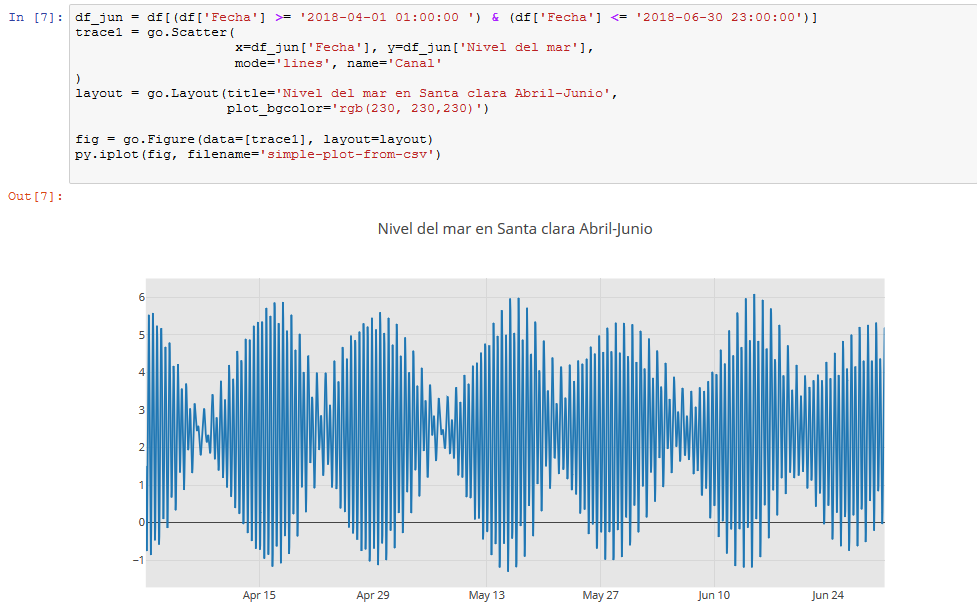
\includegraphics[width=\linewidth]{4-07.png}
\end{figure}
\begin{figure}[h]
  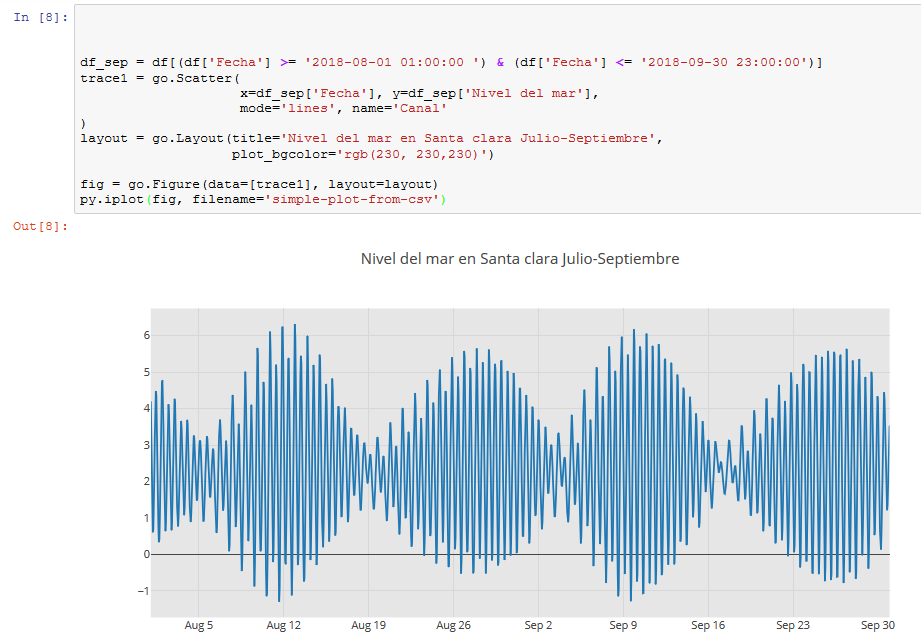
\includegraphics[width=\linewidth]{4-08.png}
\end{figure}
\clearpage

5.Para probar el análisis con transformada de Fourier, se tomaron los datos de la marea del periodo de Enero-Marzo, se graficó por medio de Plotly y se encontraron los siguientes valores en sus picos:\\ y=2.38909, y=0.8928524, y=0.581973.\\
\begin{figure}[h]
  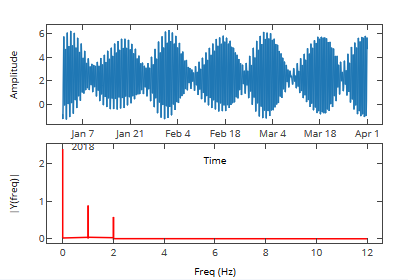
\includegraphics[width=\linewidth]{4-09.png}
\end{figure}
\clearpage
\section{Conclusiones}
El método de predicción de mareas que se utiliza es llamado "Análisis armónico" que se compone de una suma de "Constituyentes" en la forma  f(t) = H cos(at + phi) donde "H" es la amplitud, "a" la velocidad y "phi" la fase. Se han encontrado muchos de estos valores a través del tiempo y un ejemplo de ellos son:\\
\begin{figure}[h]
  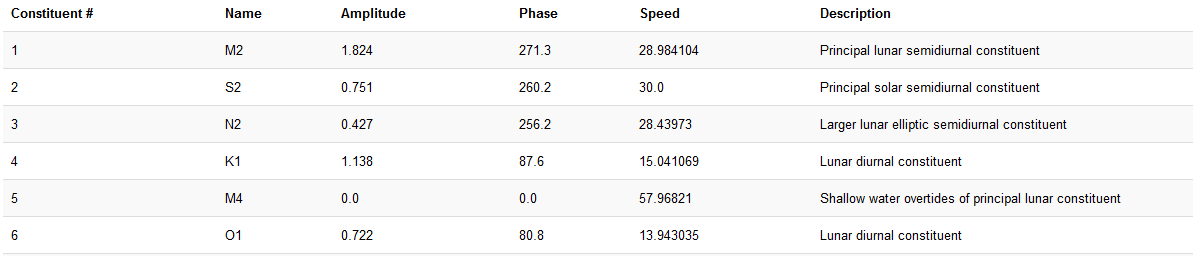
\includegraphics[width=\linewidth]{4-10.png}
\end{figure}
\\
Calculando la función f(t) de cada de una de las constituyentes se puede encontrar valores que se aproximen a los encontrados en la amplitud de la gráfica producida por la transformada de Fourier de los datos de las mareas en el Golfo de Santa Clara y así saber cuales son sus constituyentes que forman la marea para poder hacer nuestras propias predicciones.\\
Por ejemplo si calculamos que valor tendria f(t) de las constituyentes de la tabla anterior:\\
M2   1.824cos(28.984104 + 271.3) = 0.919821432\\
S2   0.751cos(30 + 260.2) = 0.259318947\\
N2   0.427cos(28.439730 + 256.2) = 0.107920119\\
K1   1.138cos()2.041069 + 87.6) = -0.249043006\\
M4   0.000cos(57.96821 + 0) = 0\\
O1   0.722cos(13.943035 + 80.8) = -0.597\\

Siguiendo asi, hay mas de 30 constituyentes que se podrian calcular para ver si algunos otros valores se aproximan mas a los encontrados en la gráfica pero la verdad actualmente con mis conocimientos no entiendo como analizar correctamente una transformada de Fourier pero me quedo con muchos ánimos para hacerlo pronto en un futuro, y tomar el objetivo de poder encontrar estos valores en los datos del manglar de Sargento.



\end{document}
